\subsection{Reconstruction level UE versus jet observables}
The reconstructed level underlying event measurement is shown via the mean transverse energy density of full calorimeter topoclusters as a function of leading jet $\pT$ in Figure~\ref{fig:reco_ue_pt}. 
Fairly good agreement is seen between data and simulation for these uncorrected distributions prior to unfolding.
\begin{figure}
    \centering
    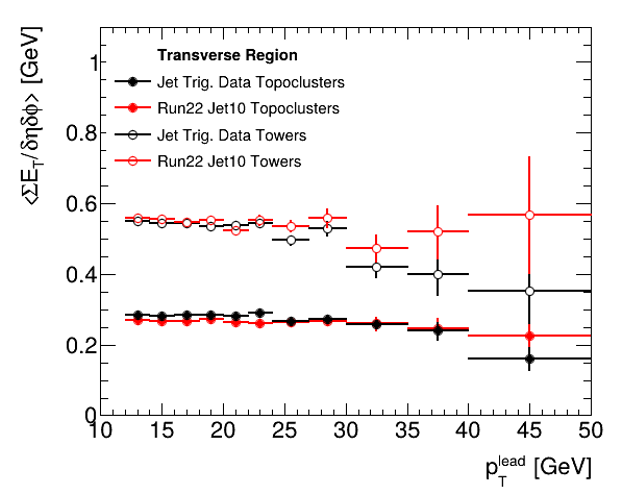
\includegraphics[width=0.7\linewidth]{ueinpp/Figures/unfolding/reco_ue_pt_transverse.png}
    \caption{Comparison of reconstructed level mean topocluster (tower) total transverse energy versus leading jet $p_{T}$ in dijet events for transverse jet regions.}
    \label{fig:reco_ue_pt}
\end{figure}

\subsection{Unfolding Procedure}
\label{sec:unfolding}

\subsubsection{Unfolding Algorithm}
An unfolding procedure is applied in the analysis to correct for detector effects such as the smearing of jet $p_{T}$ and $\Sigma E_{T}$ spectra due to calorimeter energy resolution effects. 
The procedure uses the response modeled in simulation to correct for these detector effects and extract the underlying truth spectra of the leading jet $p_{T}$ and transverse region $\Sigma E_{T}$ observables.
This mapping of truth-level information and reconstruction-level information is encoded in a response matrix derived from simulation.
Additional corrections related to the efficiency and purity of the event selection at the truth and reconstruction levels are included in the response matrix as Misses and Fakes, respectively.

The unfolding procedure used in this analysis is performed with the RooUnfold package~\cite{adye2011} and uses a Bayesian iterative unfolding method~\cite{DAGOSTINI1995487}.
The basis for this Bayesian unfolding method is the application of Bayes' theorem to an experimental distribution where $E_j$ represents a measured event and $C_i$ represents a true event or "cause"~\cite{DAGOSTINI1995487}:
\begin{equation}
    \hat{n}(C_i) = \sum_{j=1}^{n_E}M_{ij}n(E_j) \quad M_{ij} = \frac{P(E_j|C_i)P_0(C_i)}{[\sum_{l=1}^{n_E}P(E_l|C_i)][\sum_{l=1}^{n_C}P(E_j|C_l)P_0(C_l)]}
\end{equation}
where $\hat{n}(C_i)$ is the best estimate of the true distribution or distribution of "causes", $M_{ij}$ is the unfolding matrix, and $n_{E_j}$ is the measured distribution of events. 
The unfolding matrix $M_{ij}$ is comprised of the conditional probability $P(E_j|C_i)$, which is the probability of a measured event $j$ given a true cause $i$, and the prior probability $P_0(C_i)$, which is the initial guess for the true cause distribution. 
$\sum_{l=1}^{n_E}P(E_l|C_i)$ is the efficiency to measure a true cause $i$ and $\sum_{l=1}^{n_C}P(E_j|C_l)P_0(C_l)$ is the probability of measuring an event $j$ given the prior distribution.
This unfolding procedure is applied iteratively, where the unfolded distribution $\hat{n}(C_i)$ from one iteration is used as the prior for the next iteration and the change in the unfolded distribution per iteration is checked by comparing the initial expected number of truth events in each bin, $n_0(C_i) = P_0(C_i) \sum_{j=1}^{n_E}P(E_j|C_i)$, to the unfolded number of truth events in each bin, $\hat{n}(C_i)$, to determine the optimal number of iterations for the unfolding procedure.

For this analysis, the unfolding is performed in two dimensions with the leading jet $p_{T}$ and transverse region $\Sigma E_{T}$ as the two axes of the response matrix and unfolded spectra. 
The unfolding procedure corrects for detector effects such as the finite calorimeter energy resolution and the hadronic scale correction on the $\Sigma E_{T}$ observable, which is not applied at the reconstruction level.
The unfolding procedure also accounts for the trigger efficiency, timing cut efficiency and run-dependent pileup corrections applied as scale factors on the data events filling the histogram that will be used for unfolding, as these corrections are applied to the data at the reconstruction level and thus are included in the response matrix derived from simulation.

\subsubsection{Simulation Processing for Unfolding Procedure}
The response matrix used in the unfolding procedure is built from \pythia jet-triggered samples by applying the same kinematic selections used in the data and outlined in Section~\ref{sec:ueinpp_selection} to the truth and reconstructed level information. 
The reconstructed leading jets are calibrated using the JES correction function derived from a MC-based numerical inversion JES derivation~\cite{ppg09AN} and an additional JER smearing term of 10.1\% is applied to the simulation reconstruction-level jets, determined from differences in the Data/MC JER~\cite{ppg08AN}. Finally, truth and calibrated jets are matched with a matching radius requirement of $\Delta R < 0.75R$. 

The transverse region $E_{T}$ is determined by summing topocluster $E_{T}$ in the transverse region: $\pi/3 < |\Delta\phi| < 2\pi/3$ relative to the leading jet. 
Truth $\Sigma E_{T}$ uses final-state particles within $|\eta|<1.1$ and applies the per-particle energy thresholds used for the analysis (0.5~GeV for hadrons and 0.2~GeV for EM particles), again summing in the transverse region.

\subsubsection{Response Matrix Filling}

Response matrices are filled using bins in $($leading jet $p_{T}, \Sigma E_{T})$ space.
The binning used for this analysis is as follows: 
\begin{itemize}
    \item Calibrated leading jet $p_{T}$ bins: ${21, 26, 32.5, 40.5, 63.5}$ \GeV
    \item Truth leading jet $p_{T}$ bins: ${17, 21, 26, 32.5, 40.5, 63.5, 82}$ \GeV
    \item Reconstructed $\Sigma E_{T}$ bins: ${-1.08, -0.1, 0.1, 1.08, 1.97, 3.05, 4.68, 6.2, 15.0}$ \GeV
    \item Truth $\Sigma E_{T}$ bins: ${0.0, 0.5, 1.08, 1.97, 3.05, 4.68, 6.2, 15.0, 35.0}$ \GeV
\end{itemize}
Events where truth and reconstructed leading jet events are matched geometrically and both are within the binned $p_{T}$ and $\Sigma E_{T}$ ranges contribute to the response matrix, while unmatched entries and entries outside the binned ranges are recorded as fakes and misses. 
Additional requirements on the response matrix bins are applied to trim bins with low statistics and reduce the effect of statistical fluctuations in the response matrix on the unfolding result.
Bins with fewer than 10 counts for a particular triggered MC sample are trimmed in the response matrix.
Figure~\ref{fig:response_matrices_inclusive} and Figure~\ref{fig:response_matrices_dijet} show the 4D response matrix and 2D projections on the leading jet $p_{T}$ and transverse region $\Sigma E_{T}$ axes derived from simulation samples with the trimmed bin requirement for the inclusive and dijet event selections, respectively.

The response matrices show fairly diagonal structure in both the leading jet $p_{T}$ and transverse region $\Sigma E_{T}$ axes, with some off-diagonal smearing in both axes due to the steeply falling $p_{T}/E_{T}$ spectra and the finite calorimeter energy resolution.
The jet $p_{T}$ response tracks a diagonal structure with $p_{T}^{reco}/p_{T}^{truth} \sim 1$, while the $\Sigma E_{T}$ response is shifted lower than 1 ($\Sigma E_{T}^{reco}/\Sigma E_{T}^{truth} \sim 0.65-0.7$); 
The calorimeters at reconstruction-level are calibrated to the EM scale.
The MC-derived JES applied to the jet $p_{T}$ accounts for the missing hadronic energy in the calorimeter response.
However, no hadronic scale correction is applied to the $\Sigma E_{T}$ observable; therefore, the main diagonal band of $\Sigma E_{T}$ response is shifted lower than 1 ($\sim 0.65-0.7$) and the unfolding accounts for the hadronic scale correction. 
An uncertainty on the hadronic scale correction is included as a systematic uncertainty in the analysis and is described in more detail in Section~\ref{sec:ueinpp_systematic_uncertainties}
Additionally, the off-diagonal smearing in the $\Sigma E_{T}$ response is also larger than the resolution effects in the jet $p_{T}$ response, which is expected due to the larger calorimeter energy resolution at lower energies. 

\begin{figure}
    \centering
    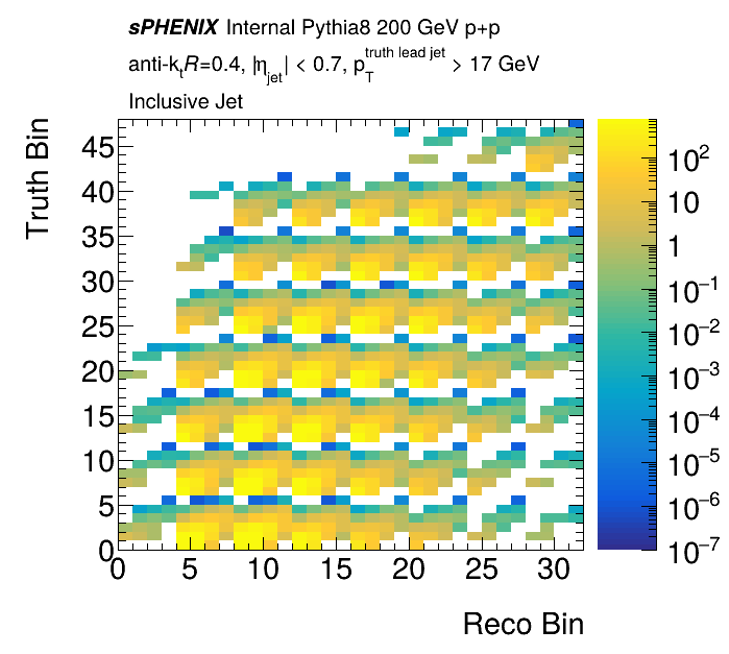
\includegraphics[width=0.7\linewidth]{ueinpp/Figures/unfolding/2D_response_matrix_inclusive.png}
    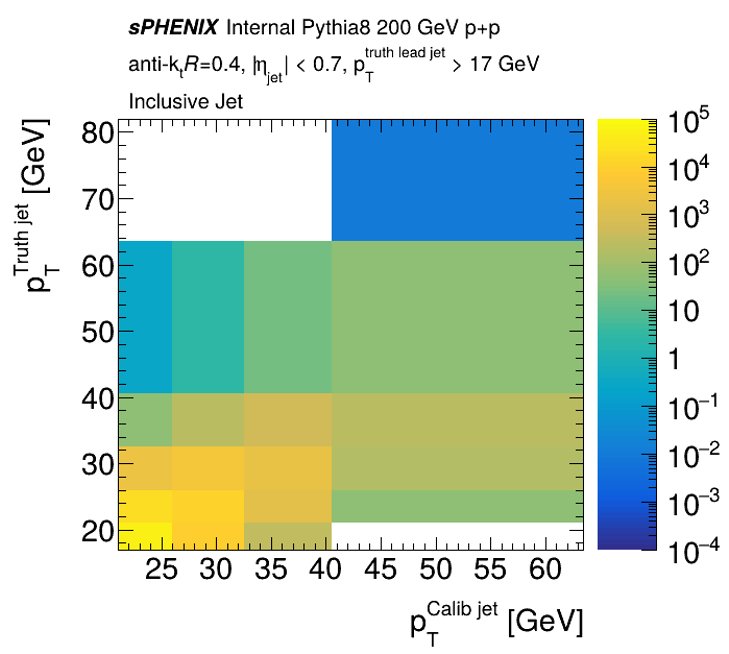
\includegraphics[width=0.48\linewidth]{ueinpp/Figures/unfolding/jetpt_response_matrix_inclusive.png}
    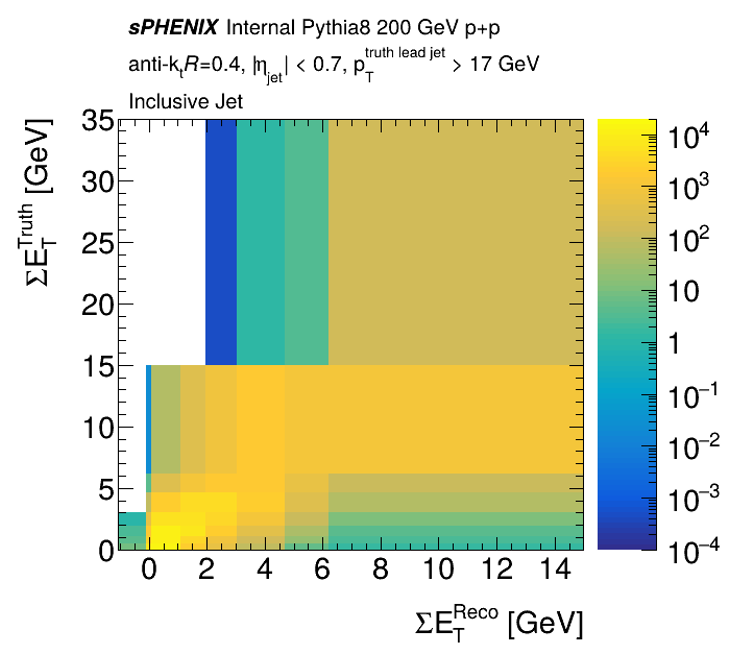
\includegraphics[width=0.48\linewidth]{ueinpp/Figures/unfolding/caloet_response_matrix_inclusive.png}
    \caption{Response matrices derived from \pythia simulation samples for inclusive jet result. The full 4D response matrix is shown with composite binning in the top plot for inclusive jet events. The 2D projections of this response matrix projected onto the leading jet $p_{T}$ (bottom left) and transverse region $\Sigma E_{T}$ (bottom right) are also shown for inclusive jet events.}
    \label{fig:response_matrices_inclusive}
\end{figure}

\begin{figure}
    \centering
    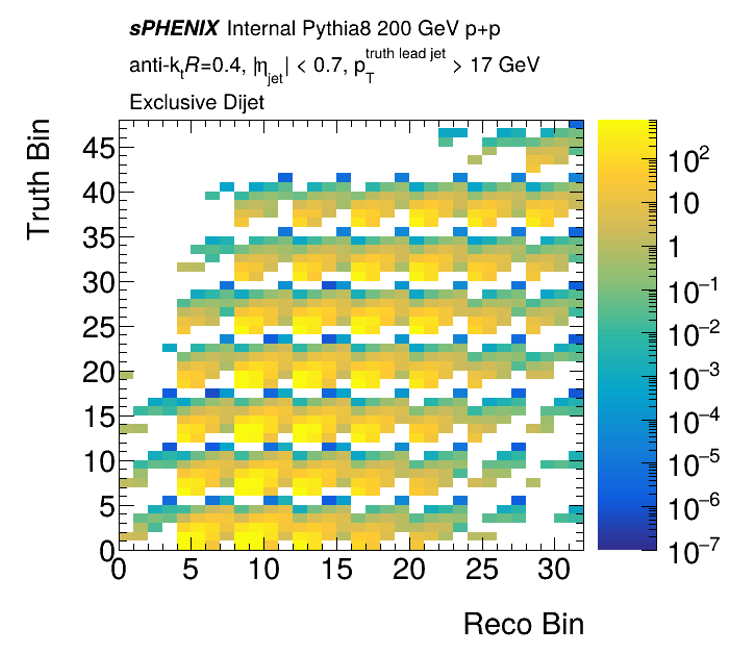
\includegraphics[width=0.7\linewidth]{ueinpp/Figures/unfolding/2D_response_matrix_dijet.png}
    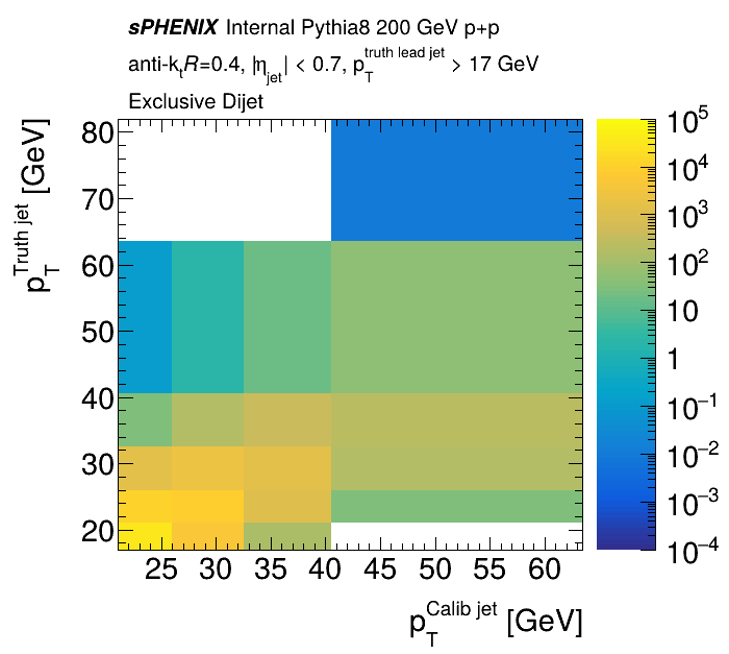
\includegraphics[width=0.48\linewidth]{ueinpp/Figures/unfolding/jetpt_response_matrix_dijet.png}
    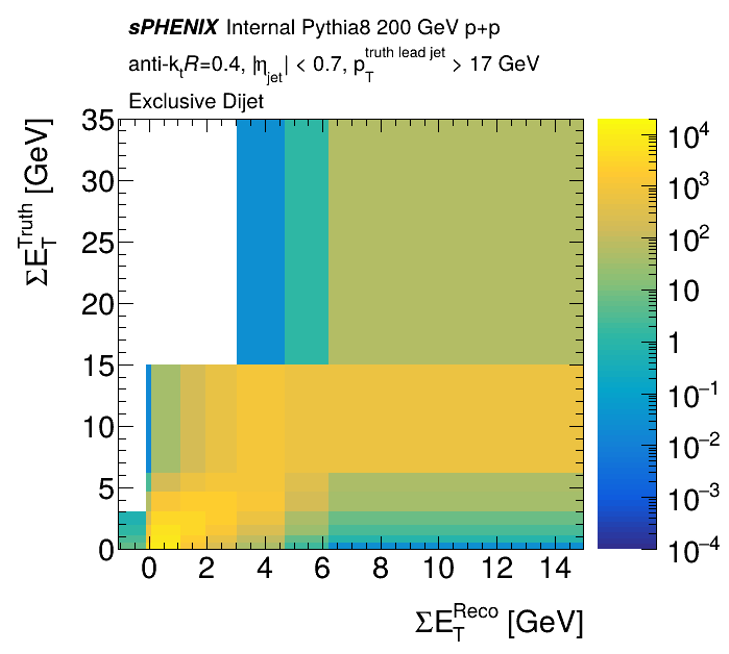
\includegraphics[width=0.48\linewidth]{ueinpp/Figures/unfolding/caloet_response_matrix_dijet.png}
    \caption{Response matrices derived from \pythia simulation samples for dijet result. The full 4D response matrix is shown with composite binning in the top plot for dijet events. The 2D projections of this response matrix projected onto the leading jet $p_{T}$ (bottom left) and transverse region $\Sigma E_{T}$ (bottom right) are also shown for dijet events.}
    \label{fig:response_matrices_dijet}
\end{figure}

\subsubsection{MC Prior Reweighting for Unfolding}
\label{sec:prior_reweighting}
To reduce prior dependence in the unfolded result, the simulation truth distributions are reweighted to match a data-driven pseudo-truth spectrum. 
The procedure uses the simulation response matrices and the data measured spectrum as inputs to a single-iteration RooUnfoldBayes pre-unfolding. 
For each response matrix variation, nominal and each systematic variation, the unfolded pseudo-truth is normalized and divided by the normalized simulation truth to form a weight matrix. 
These weights are applied to the original truth distribution to produce reweighted truth spectra that serve as priors for the subsequent response-matrix reweighting step. 

\begin{figure}
    \centering
    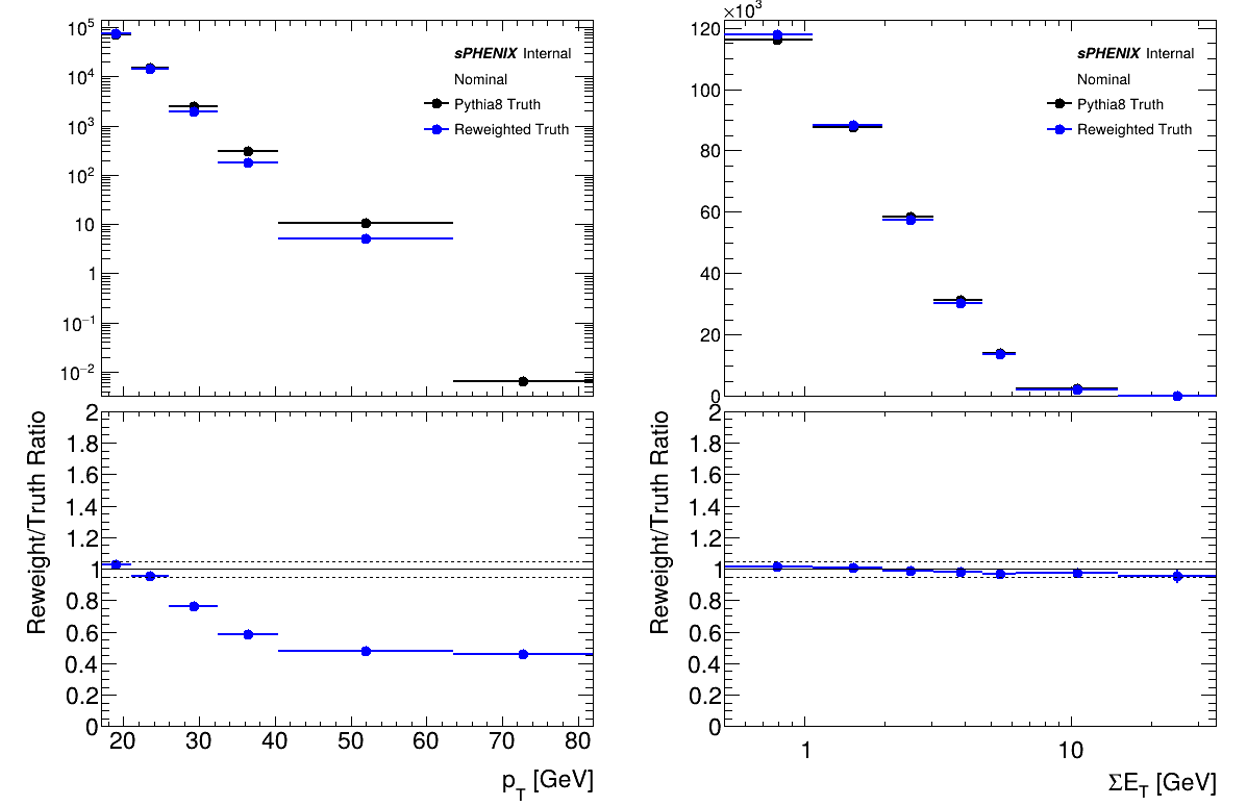
\includegraphics[height=0.4\textheight]{ueinpp/Figures/unfolding/prior_reweighting_inclusive.png}
    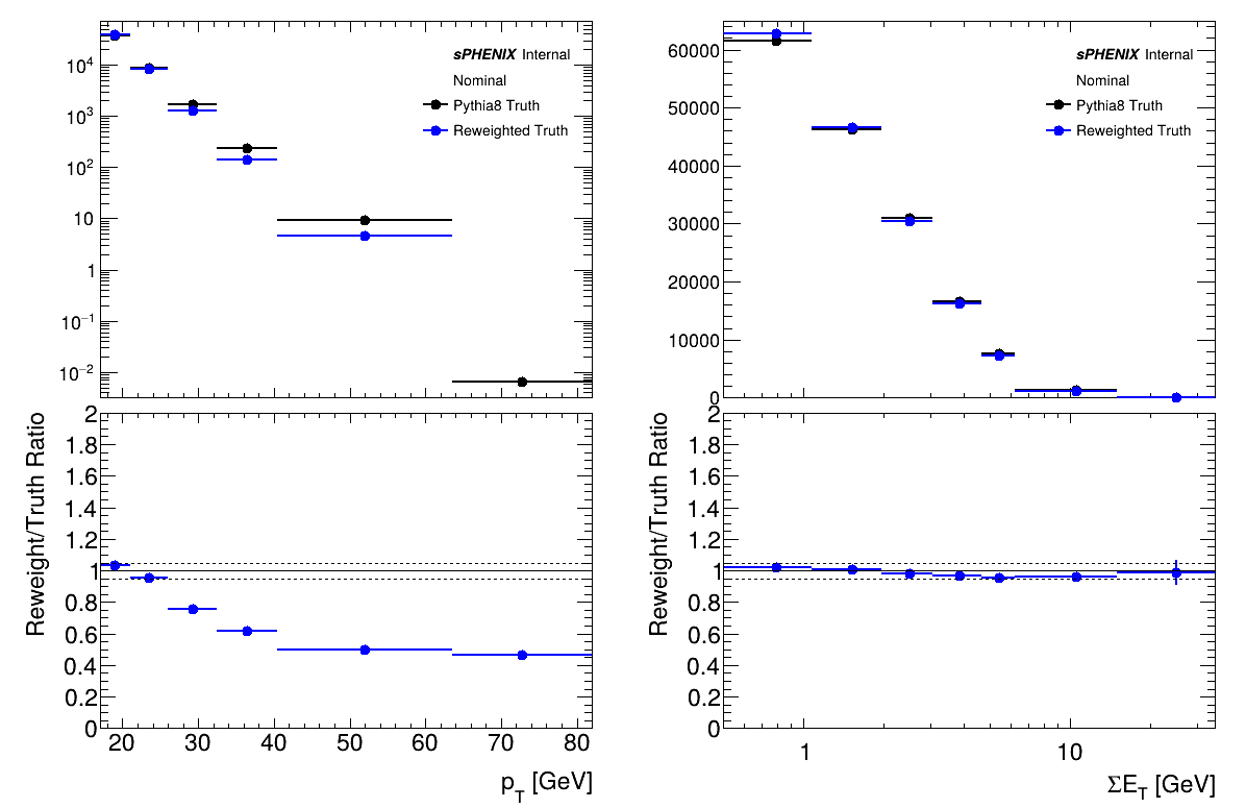
\includegraphics[height=0.4\textheight]{ueinpp/Figures/unfolding/prior_reweighting_dijet.png}
    \caption{Prior reweighting truth distributions for inclusive jet (top) and dijet (bottom) events. Projections onto the leading jet $p_{T}$ (left) and transverse region $\Sigma E_{T}$ (right) distribution axes before and after the full 2D prior reweighting for the nominal response matrix are shown.}
    \label{fig:prior_reweighting_truth}
\end{figure}

\subsubsection{Closure Tests}
Closure tests are performed with the same response matrices used in the unfolding. 
Both a full-closure test, where each response matrix is unfolded against its own measured distribution with one Bayesian iteration, and a half-closure test, where the response from one half-sample is used to unfold the measured distribution from the complementary half-sample across 1--6 iterations, are performed. 
All response matrices are tested for closure. 
Statistical uncertainties on the closure spectra are evaluated with 1000 toy variations of the response matrix and combined in quadrature with the unfolded errors. 
The full closure and half closure tests for the nominal response matrix are shown in Figures~\ref{fig:full_closure_test_dijet} and \ref{fig:half_closure_test_dijet}. Both the full and half closure tests show agreement between the truth spectra and unfolded spectra of unity within statistical uncertainties. 
Since both closure tests fully close, there is no additional systematic taken for non-closure in the unfolding procedure.

\begin{figure}
    \centering
    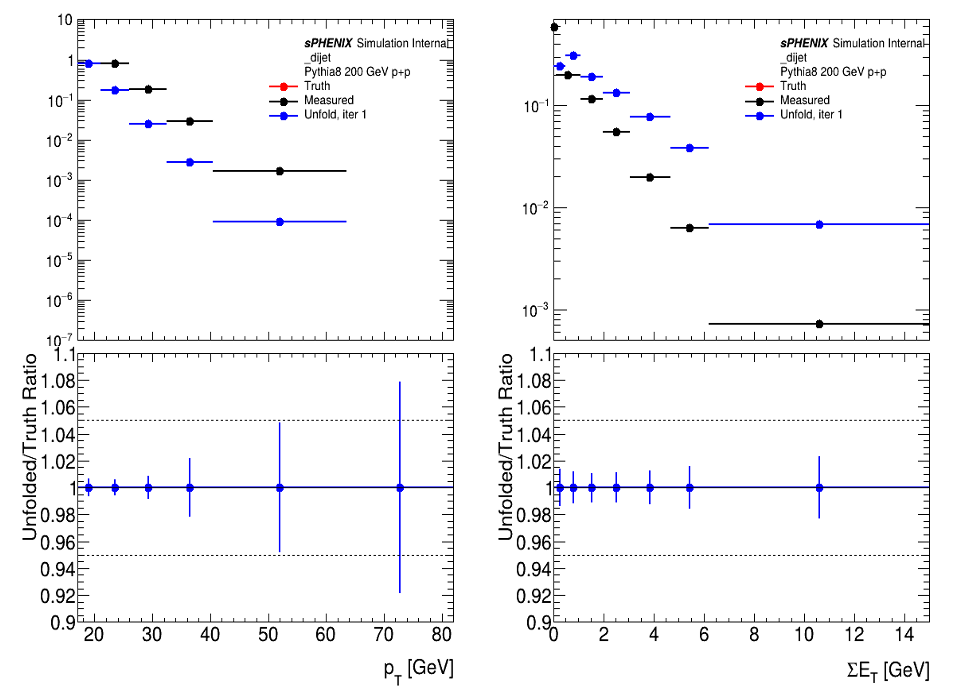
\includegraphics[height=0.45\textheight]{ueinpp/Figures/unfolding/dijet_full_closure.png}
    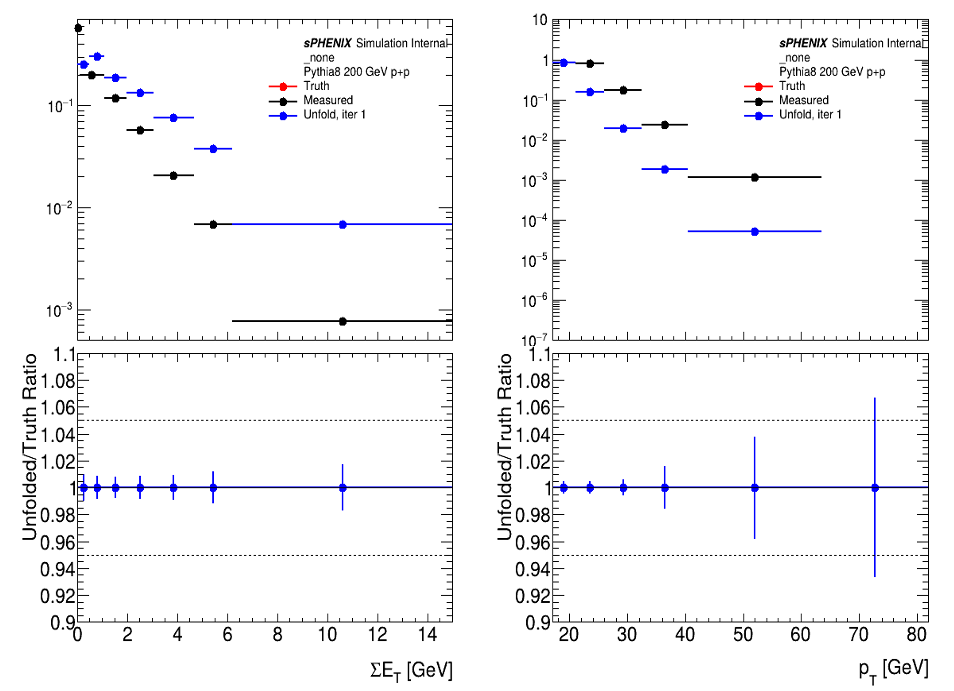
\includegraphics[height=0.45\textheight]{ueinpp/Figures/unfolding/inclusive_full_closure.png}
    \caption{Full-closure test results for dijet (top) and inclusive jet (bottom) events. The plots show both the truth, measured, and unfolded spectra for the reweighted and trimmed response matrices and below the unfolded-to-truth ratios for both jet $p_{T}$ (left) and transverse $\Sigma E_{T}$ (right).}
    \label{fig:full_closure_test_dijet}
\end{figure}

\begin{figure}
    \centering
    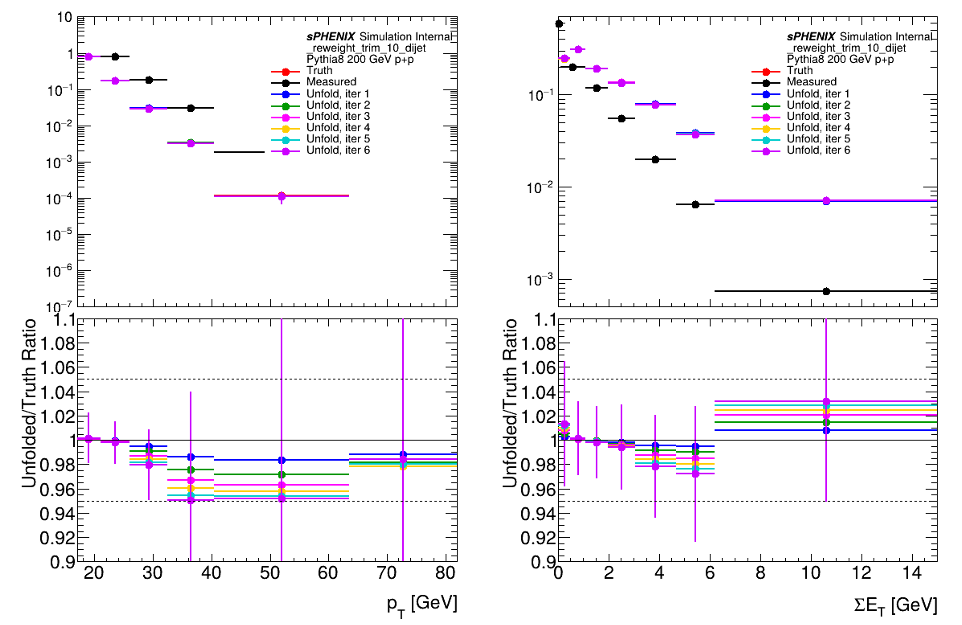
\includegraphics[height=0.45\textheight]{ueinpp/Figures/unfolding/dijet_half_closure.png}
    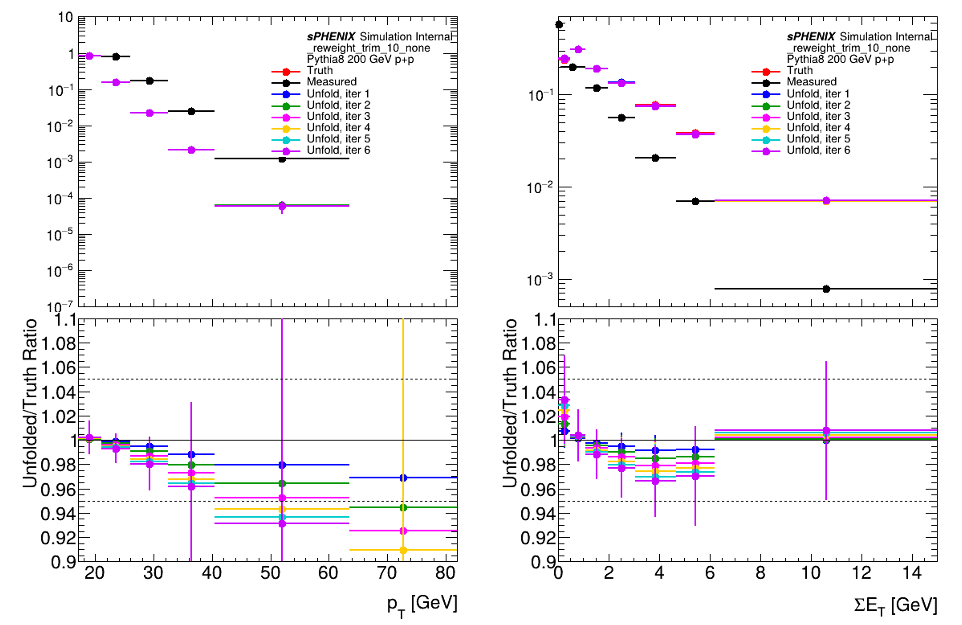
\includegraphics[height=0.45\textheight]{ueinpp/Figures/unfolding/inclusive_half_closure.png}
    \caption{Half-closure test results for dijet (top) and inclusive jet (bottom) events. The plots show both the truth, measured, and unfolded spectra for the reweighted and trimmed response matrices and below the unfolded-to-truth ratios for both jet $p_{T}$ (left) and transverse $\Sigma E_{T}$ (right).}
    \label{fig:half_closure_test_dijet}
\end{figure}

\subsubsection{Data Processing for Unfolding Procedure} 
Reconstruction-level histograms of $($leading jet $p_{T}, \Sigma E_{T})$ spectra that are later unfolded are built from data using the event selections outlined in Section~\ref{sec:ueinpp_selection}.
The leading jet $p_{T}$ in the data is then calibrated with the same MC-derived JES correction applied to the simulation reconstruction-level jets, and trigger efficiency, timing cut efficiency and run-dependent pileup corrections are applied as scale factors on the data events filling the histogram that will be used for unfolding.

\subsubsection{Unfolding Data Results}
A 2D unfolding procedure in leading jet $p_{T}$ and transverse region $\Sigma E_{T}$ is performed using the 4D response matrices from simulation and the 2D histograms of reconstruction-level information from data.
The unfolding is performed with the response matrices from simulation after both the trimming requirements and prior reweighting procedure for up to 20 iterations to determine the optimal number of iterations in the unfolding process
where the change in unfolded result per iteration is at the level of the statistical precision of the measurement. 

Figure~\ref{fig:unfold_iterations} shows this iteration optimization point for unfolding both inclusive jet and dijet event using the nominal-result MC response matrix with a trimming requirement of 10 entries for each jet triggered MC sample and the prior reweighting procedure applied.
The two trends which define this minimum is the total change in unfolded values for each iteration in red and the total statistical error on the unfolded result in blue determined from the quadrature sum of the bin errors in the data histogram and the effect of statistical error in the response matrix tested by sampling 1000 toy models varying the response matrix bin values within 1$\sigma$ of their nominal value.
For both the inclusive jet and dijet results, the change in unfolded values per iteration x total statistical error curve has a minimum around 3 iterations, and thus 3 iterations is chosen as the optimal point for unfolding to balance minimizing prior dependence with minimizing statistical uncertainty in the measurement.
\begin{figure}
    \centering
    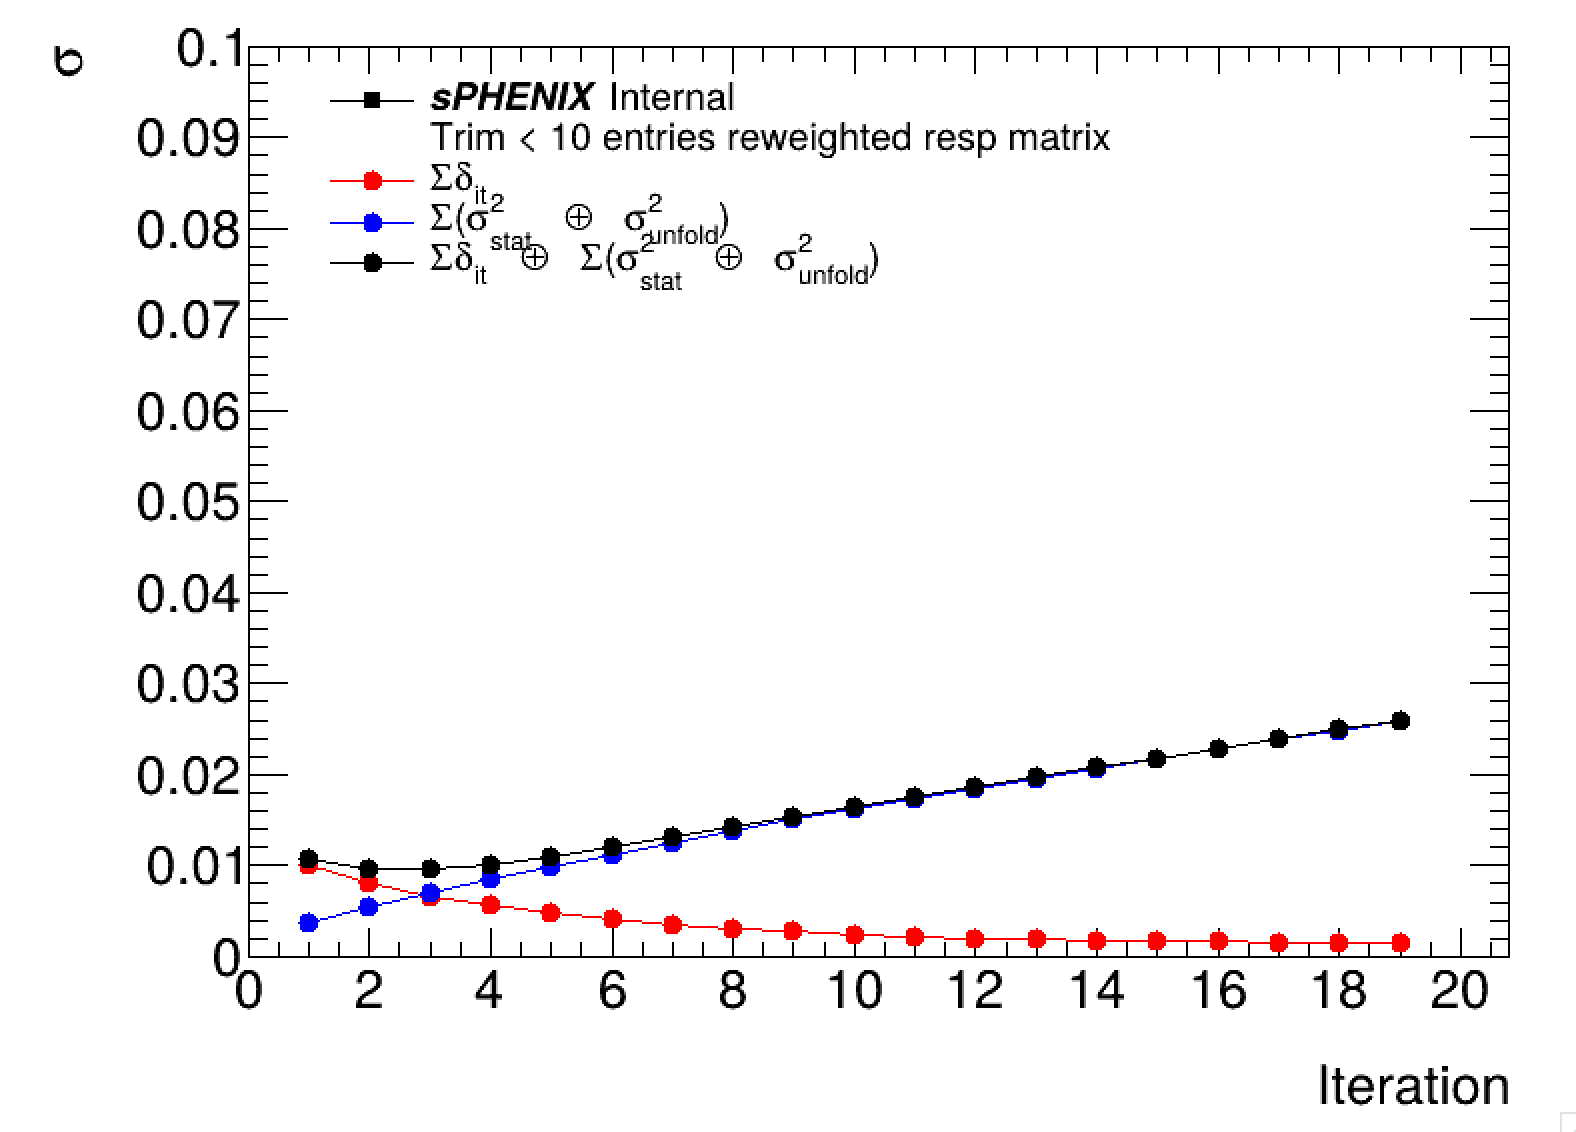
\includegraphics[width=0.48\linewidth]{ueinpp/Figures/unfolding/unfolding_iterations_inclusive.png}
    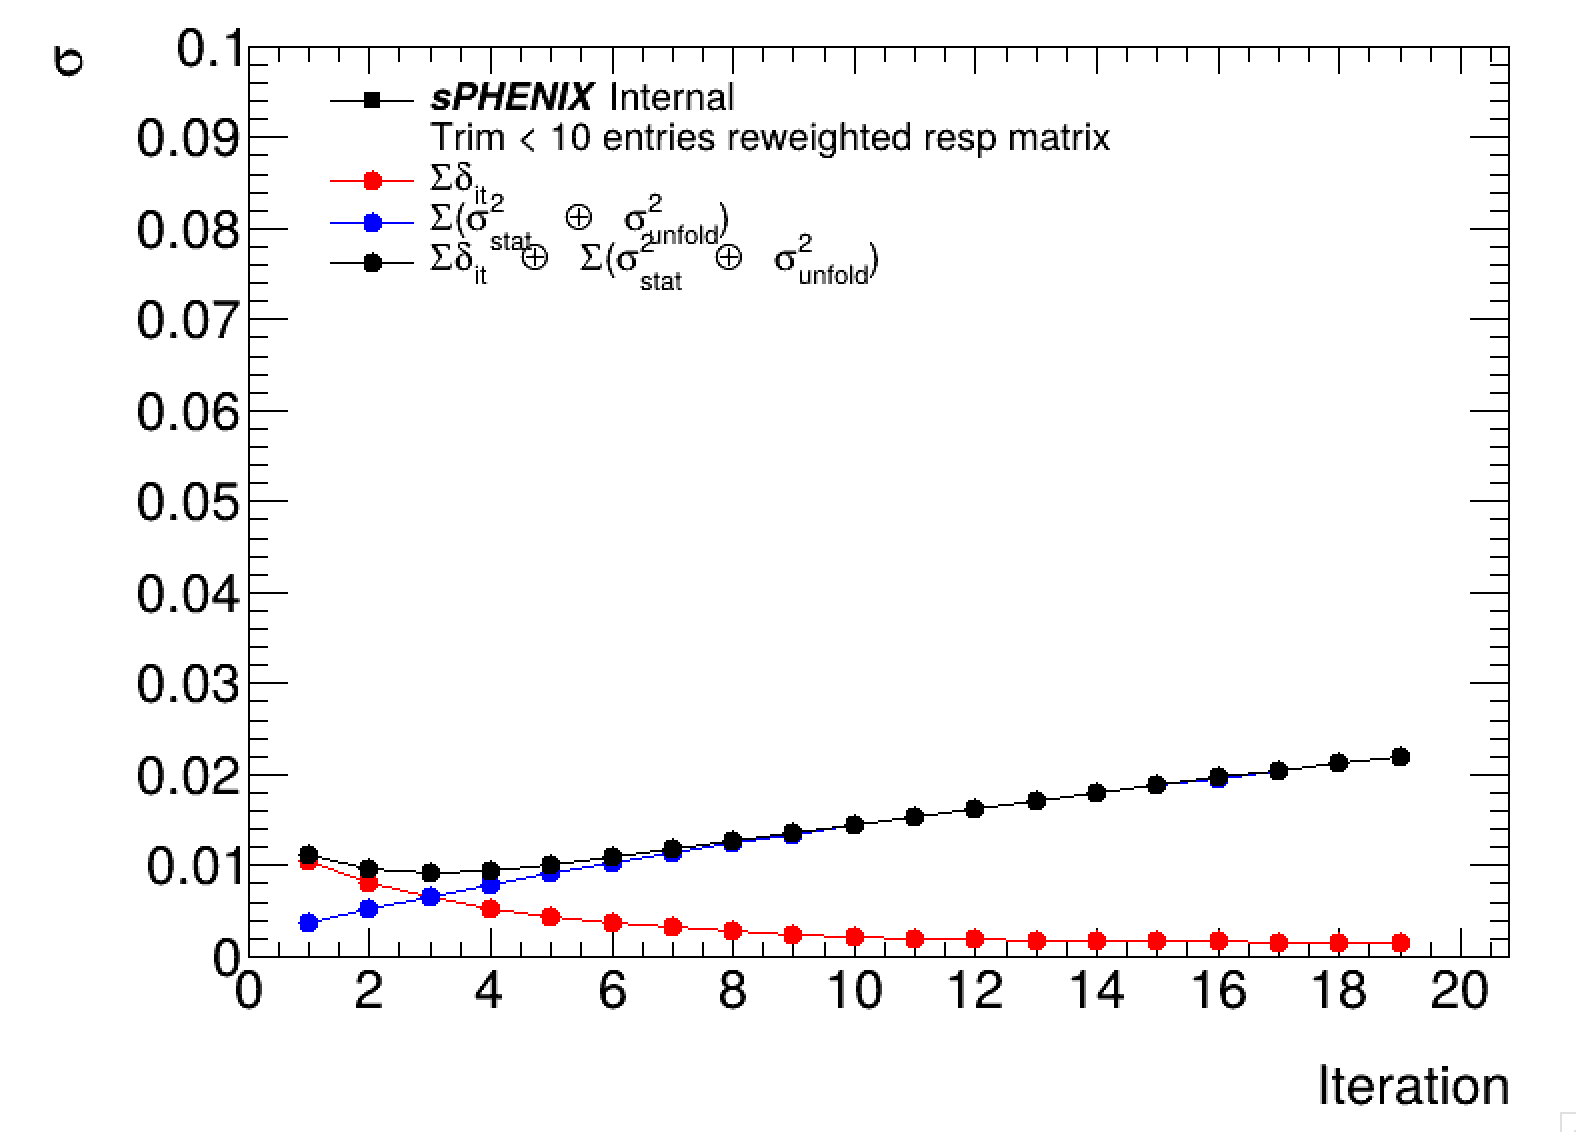
\includegraphics[width=0.48\linewidth]{ueinpp/Figures/unfolding/unfolding_iterations_dijet.png}
    \caption{Overall stability of unfolding procedure as a function of unfolding iterations for inclusive jet (left) and dijet (right) results. Total change in unfolded result per iteration shown red. Total statistical error in unfolded result per iteration shown in blue.}
    \label{fig:unfold_iterations}
\end{figure}
